\section{Background}
\label{background}

This section briefly reviews essential background on vehicular security and message authentication codes. 
The experienced reader may wish to skip to Section~\ref{problem}. 
We assume the reader is familiar with cryptographic hash functions as explained, for example, 
by Stinson~\cite{Stinson} and NIST~\cite{FIPS-180-4}.

\subsection{ECUs}
Electronic Control Units (ECUs) found in an automotive computer network are low-power, single-purpose devices. ECUs on the CAN bus control many components in a modern automobile, from headlights and window controls, to brakes and engine. They are not typically designed with security in mind and frequently comprise a basic CAN bus transceiver, basic message processor, and an actuator. The message processor identifies whether or not a message being broadcast is interesting to the ECU and arbitrates bus rights with the other ECUs. 

\subsection{The CAN Bus}
The CAN bus is a simple, low-speed bus designed to network simple nodes. In an automotive environment, 
it typically runs at 500~kbps.\footnote{kilobits per second (kbps).} As shown in Figure~\ref{fig-frame}, 
a frame contains an 11-bit identifier field and 
a data payload, as well as some control bits. Figure~\ref{fig-frame} shows the data payload as 8~bits, but
it can be 8 to 64~bits and is typically 64~bits. [ref?]
The payload of up to 8~bytes is the most important element, as any MAC must fit into this frame or use a more complex multi-frame data transmission protocol that may or may not be supported on all ECUs. 

We use the term ``message'' to refer to the data payload of one logical transmission.
Any payload longer than 64~bits must be sent as a multi-frame transmission.

% we need agreement on terminology.  Do we instead want to use "multi-frame message" ?
% is there an industry convention?

Ideally, and in the case of Mini-MAC, the MAC tag
can fit into the payload together with the data, thus not increasing bus utilization. 
In test data captured by the authors from a 2010 Toyota Prius, 
approximately 61\% of messages contain at most four data bytes
(20\% contain 4~bytes; 16\% contain 3~bytes; 17\% contain 2~bytes; and 8\% contain 1~byte).
Approximately 35\% of messages contain a full 8~data bytes, and 4\% contain 7~bytes.
Thus, for most messages, there are at least four bytes of space available for a MAC tag.

We observed approximately 25 messages sent per second on average (40 maximum per second).

% 25 ms between msgs
% can you describe the distribution of available space more thoroughly?
% 35% percent of messages were the full 8 bytes. 4% were 7 bytes, 
% and the remaining 61% that are 4B or less are 20% 4 bytes, 16% 3 bytes, 17% 2 bytes and 8% 1 byte.

	\begin{figure*}
		\centering
		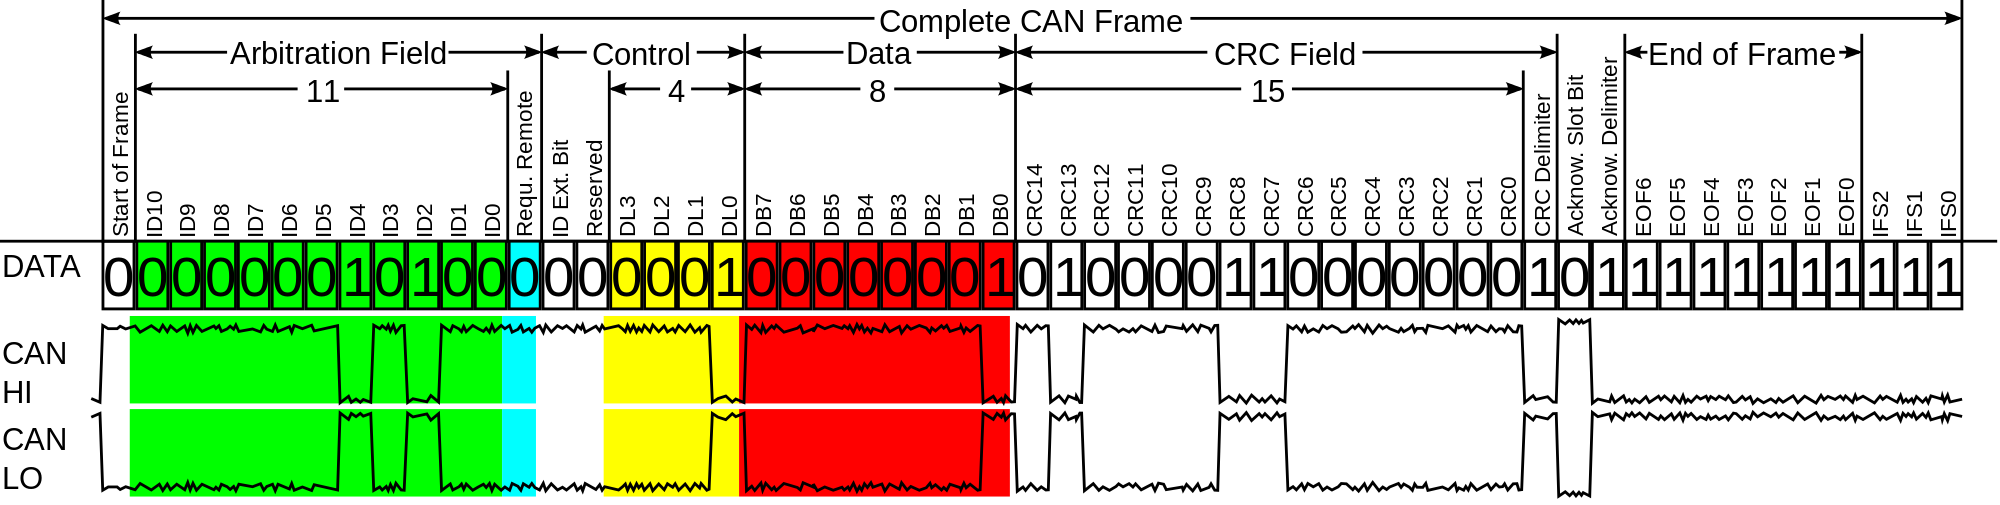
\includegraphics[width=\linewidth]{figures/can_frame.png}
		\caption{The CAN frame~\cite{?} [need to cite fig].  
		Each transmission on the CAN bus is a structured sequence of 55--111~bits including 8--64 data~bits.}
		\label{fig-frame}
	\end{figure*}

\subsection{Bus Access}

To spoof or replay messages on the CAN bus, the attacker must have access to it.
There are several ways to access the CAN bus:  (1) There is a
physical connection through the On-Board Diagnostic (OBD-II) port, 
typically located underneath the steering wheel.  An attacker might hide
access to this port by splicing into unexposed wires.
(2) An attacker might corrupt an ECU by rewriting its firmware. An attacker might
do so while the car is being serviced or by entering the car while it is parked.
(3) An attacker might gain access to the CAN bus by exploiting or corrupting a peripheral
device connected to it, such as a cellular phone, audio system, or Bluetooth
radio.  For example, Checkowa~\cite{Checkoway-2011} gained bus access by packing 
malware into a WMA audio file played on the car stereo. [give another example
of wireless access from drive-by attacker]

Despite many demonstrated security flaws, automotive 
manufacturers have been unreasomnably hesitant to acknowledge the vulnerabilities inherent to the CAN bus,
sometimes wishfully claiming that undetected bus access is difficult. 

%[do you have a cite? for example,
%a quote from a car manufacturer saying something ridiculous?]

\subsection{Message Authentication Codes}

Given a message and optionally a key, a Message Authentication Code (MAC) computes a short string (called a tag) 
that a recipient can use, together with the message, to verify the authenticity of the message.  The recipient 
verifies the tag by recomputing it.

The Keyed-Hash Message Authentication Code (HMAC)~\cite{HMAC,FIPS-198-1} 
is a well-known MAC construction that keys an underlying component hash function.  
Breaking it is as hard as breaking the component hash function.

HMAC is computed as

\begin{equation}
H((k\oplus \text{opad})\concat H((k\oplus \text{ipad})\concat \text{message})) ,
\end{equation}

\noindent
where $k$ is the key, and opad and ipad are the outer and inner hash padding strings, respectively. 
These strings are constant strings defined by 0x5C and 0x36, repeated until the hash input is of the appropriate length. 
$H$ is the component hash function used. 
The symbols $\oplus$ and $\concat$ represent exclusive-or (XOR) and concatenation, respectively.

%\subsection{Car-to-X}


